\documentclass{article}
\usepackage{graphicx} % Required for inserting images
\usepackage[utf8]{inputenc}
\usepackage{amsmath,amsfonts,amssymb,amsthm}
\usepackage{enumerate,bbm}
\usepackage{leftindex}
\usepackage{tikz,tikz-cd,graphicx,color,mathrsfs,color,hyperref,boldline}
\usepackage{caption,float}
\usepackage[a4paper,margin=1in,footskip=0.25in]{geometry}

\usepackage{listings}
\usepackage{xcolor}

\usepackage{tabularx,capt-of}

\usepackage{blindtext}
%Image-related packages
\usepackage{graphicx}
\usepackage{subcaption}
\usepackage[export]{adjustbox}
\usepackage{lipsum}

%hyperref setup
\hypersetup{
    colorlinks=true,
    linkcolor=blue,
    filecolor=magenta,      
    urlcolor=cyan,
    pdftitle={Overleaf Example},
    pdfpagemode=FullScreen,
    }

%New colors defined below
\definecolor{codegreen}{rgb}{0,0.6,0}
\definecolor{codegray}{rgb}{0.5,0.5,0.5}
\definecolor{codepurple}{rgb}{0.58,0,0.82}
\definecolor{backcolour}{rgb}{0.95,0.95,0.92}

%Code listing style named "mystyle"
\lstdefinestyle{mystyle}{
  backgroundcolor=\color{backcolour}, commentstyle=\color{codegreen},
  keywordstyle=\color{magenta},
  numberstyle=\tiny\color{codegray},
  stringstyle=\color{codepurple},
  basicstyle=\ttfamily\footnotesize,
  breakatwhitespace=false,         
  breaklines=true,                 
  captionpos=b,                    
  keepspaces=true,                 
  numbers=left,                    
  numbersep=5pt,                  
  showspaces=false,                
  showstringspaces=false,
  showtabs=false,                  
  tabsize=2
}

%"mystyle" code listing set
\lstset{style=mystyle}

\theoremstyle{definition}
\newtheorem{defn}{Definition}[section]
\newtheorem{example}[defn]{Example}
\theoremstyle{remark}
\newtheorem{rem}{Remark}
\newtheorem{remS}[section]{defn}
\theoremstyle{plain}
\newtheorem{lem}[defn]{Lemma}
\newtheorem{thm}[defn]{Theorem}
\newtheorem{prop}[defn]{Proposition}
\newtheorem{fact}[defn]{Fact}
\newtheorem{crly}[defn]{Corollary}
\newtheorem{conj}[defn]{Conjecture}

%\newtheorem*{programming*}{Programming Task}

%\newtheorem{innercustomgeneric}{\customgenericname}
%\providecommand{\customgenericname}{}
%\newcommand{\newcustomtheorem}[2]{%
%  \newenvironment{#1}[1]
%  {%
%   \renewcommand\customgenericname{#2}%
%   \renewcommand\theinnercustomgeneric{##1}%
%   \innercustomgeneric
%  }
%  {\endinnercustomgeneric}
%}

%\newcustomtheorem{question}{Question}
%\newcustomtheorem{programming}{Programming Task}

\newcommand{\NN}{\mathbb{N}}
\newcommand{\ZZ}{\mathbb{Z}}
\newcommand{\QQ}{\mathbb{Q}}
\newcommand{\RR}{\mathbb{R}}
\newcommand{\CC}{\mathbb{C}}
\newcommand{\PP}{\mathbb{P}}
\newcommand{\FF}{\mathbb{F}}
\newcommand{\Hom}{\operatorname{Hom}}
\newcommand{\im}{\operatorname{im}}
\newcommand{\id}{\operatorname{id}}
\newcommand{\Ind}{\operatorname{Ind}}
\newcommand{\Res}{\operatorname{Res}}
\newcommand{\btop}{\mathbf{Top}}
\newcommand{\bdel}{\mathbf{\Delta}}
\newcommand{\sing}{\operatorname{Sing}}
\newcommand{\bset}{\mathbf{Set}}
\newcommand{\Rmod}{\mathbf{Mod}_R}

\newcommand{\calD}{\mathcal{D}}

\newcommand{\sol}{\textit{Solution: }}

\title{Simplicial Homotopy Theory}
\author{Kevin}
\date{January 2025}

\begin{document}
\maketitle
\section{Introduction}
Recall basic notions from category theory
\begin{defn}
    A category $\mathscr{C}$ consists of a collection of objects, denoted $\operatorname{ob}(\mathscr C)$, and for each pair of objects $A,B$, a collection of morphisms $\Hom_{\mathscr C}(A,B)$ such that
    \begin{itemize}
        \item [(i)] There is an associative composition law of morphisms.
        \item[(ii)] For each $A\in\operatorname{ob}(\mathscr C)$, there is a distinguished element $\id_A\in\Hom_{\mathscr C}(A,A)$, which is left and right unital.
    \end{itemize}
\end{defn}
\begin{defn}
    A morphism is called an isomorphism if it has a two-sided inverse.
\end{defn}

Given a category $\mathscr{C}$, want to classify objects up to isomorphism.

For the purpose of this course, $\mathbf{Top}$ will denote the category  with objects those topological spaces that are homeomorphic to a CW complex. Morphisms are cts functions. Isomorphisms are homeomorphisms. We might attempt to classify objects in $\mathbf{Top}$ up to homeo.

A useful tool is a functor, for every integer $i$ and commutative irng $R$
\[H_i(-;R):\mathbf{Top}\to\Rmod,\ X\mapsto H_i(X;R)\]
A key ingredient in the defns of these functors is the study of cts maps from the n-simplex into $X$, as $n$ varies.

There is a factorization of functors.
\[H_i(-;R):\mathbf{Top}\to \mathbf{HoTop}\to\Rmod\]
where $\mathbf{HoTop}$ is the full subcategory of $\mathbf{Top}$ obtained by forcing homotopic cts maps to be equal (so an isomoprhism in this category is a htpy equivalence). Homotopy theory is the study of $\mathbf{HoTop}$.
\begin{rem}
    Isomorphism classes in $\mathbf{HoTop}$ can be understood via the moduli stack of formal groups and other objects in arithmetic geometry.
\end{rem}

\textbf{Question: How to think about objects in $\mathbf{HoTop}$ up to isomorphism?}

Roughly, a homotopy type consists of 
\begin{itemize}
    \item A collection of objects
    \item For every pair of objects a collection of isomorphism between them
    \item For every pair of parallel isomorphism $f,g:A\to B$ a collection of 2-isomorphisms between them.
\end{itemize}
\begin{example}
    The following shows two different homotopy types.
    \begin{figure}[H]
        \centering
        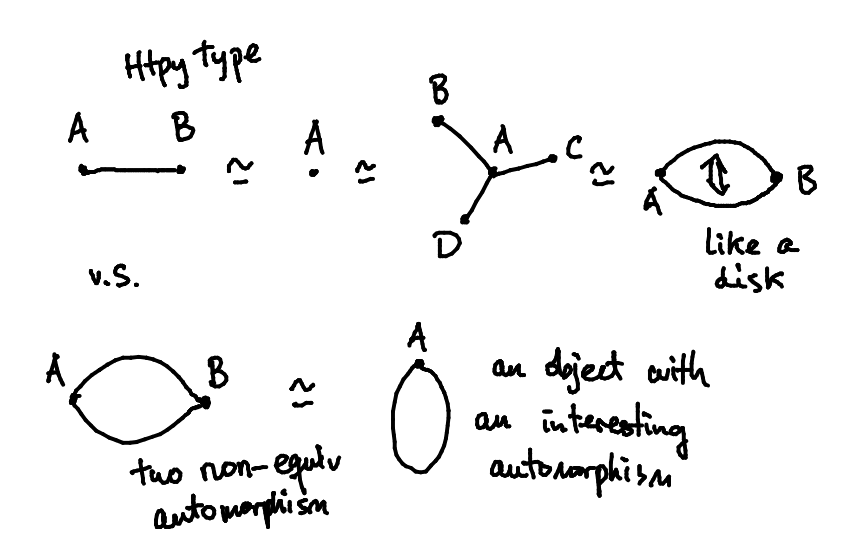
\includegraphics[width=0.5\linewidth]{Lent/pictures/htpy_type_example.PNG}
        \caption{Two different homotopy types}
        \label{fig:1}
    \end{figure}
    On the top, we have a homotopy type consisting of two objects $A, B$ and an isomorphism between them (represented by the edge). This is isomorphic to a single object $A$ as we can (formally) contract the isomorphism to identify equivalent objects. It is also equivalent to a htpy type consisting of $A,B,C,D$ where $B,C,D$ are all isomorphic to $A$ via a unique isomorphism. It is also euqivalent to the htpy type consisting of two objects $A,B$, two isomorphisms $A\to B$ and a 2-isomorphism, i.e., an equivalence of these two isomorphisms.

    On the bottom, we have another homotopy type with two objects and two non-equivalent isomorphisms. We may contract one isomoprhism and get a htpy type of consisting of a single object with an interesting automorphism.

    Sets are homotopy types with no non-trivial isomoprhisms or 2-isomorphisms.

    Groupoids, i.e., categories in which all morphisms are isomorphisms, are homotopy types with no non-trivial 2-isomorphisms and 3-isomorphisms, etc.
\end{example}
Given a topological space $X$, there is an associated homotopy type s.t.
    \begin{itemize}
        \item points of $X$ are objects. (cts maps from the $0$-simplex)
        \item paths in $X$ are isomorphisms. (cts maps from the $1$-simplex)
        \item A cts function $|\Delta^2|\to X$ is a 2-isomorphism. (Regard the map restricted to two edges of $|\Delta^2|$ as a concatenation of paths, then the map is essentially a homotopy rel the boundary of $|\Delta^1|$.)
    \end{itemize}

We want to study homotopy types. These can be presented as topological spaces (that are homeo to CW complexes) up to homotopy equivalence. SInce spaces are complicated unwieldy objects, we will seek to describe homotopy types in combinatorial terms. We will desribe homotopy types as special sorts of simplicial sets up to an appropriate notion of equivalence.

\begin{defn}
    The simplex category $\mathbf{\Delta}$ has 
    \begin{itemize}
        \item objects $[n]$ for every integer $n\ge 0$
        \item A morphism $[n]\to[m]$ is an order preserving function from $\{1\le2\le...\le n\}\to\{1\le 2\le...\le m\}$.
    \end{itemize}
\end{defn}
There is a functor $\mathbf{\Delta}\to\mathbf{Top}$ sending $[n]\mapsto|\Delta^n|$. This is a good way to visualize $\bdel$. We introduce some special notations for certain morphisms in $\bdel$.
\begin{itemize}
    \item Face maps: $\delta^i:[n-1]\to[n]$ is the order preserving injection that omits $i$.
    \item Degeneracy maps: $\sigma^i:[n+1]\to[n]$ is the order preserving surjection that hits $i$ twice.
\end{itemize}
\begin{rem}
    Every morphism in $\bdel$ is a composite of face and degeneracy maps.
\end{rem}

\begin{defn}
    A simplicial set is a functor $\mathbf{\Delta}^{op}\to\mathbf{Set}$. A morphism of simplicial sets is a natural transformation. There is a category of simplicial sets, denoted $s\bset$.
\end{defn}
Explicitly, a simplicial set $X:\bdel^{op}\to \bset$ is a collection of sets $X_0,X_1,X_2,...$, where $X_i=X([i])$ with maps of sets $d_0,...,d_n:X_n\to X_{n-1}$ and $s_0,...,s_n:X_{n}\to X_{n+1}$ satisfying the following simplicial identities:
\begin{align*}
    &d_id_j=d_{j-1}d_i,\ \ i<j\\
    &d_is_j=s_jd_{i-1},\ \ i<j\\
    &d_is_j=s_{j}d_{i+1},\ \ i>j+1\\
    &s_is_j=s_{j+1}s_i,\ \ i<j
\end{align*}
\begin{example}
    If $X$ is a topological space, there is an associated simplicial set $\sing(X):\mathbf{\Delta}^{op}\to \mathbf{Set}$ which sends $[n]$ to the set of continuous functions $|\Delta^n|\to X$. So $\sing(X)_n=\Hom_{\btop}(|\Delta^n|,X)$.
\end{example}
\begin{rem}
    Not every simplicial set is $\sing$ of some topological space. $C_\ast^{\sing}(X;R)$ depends only on $\sing(X)$.
\end{rem}

\begin{defn}
    For every integer $n\ge 0$, there is a simplicial set denoted $\Delta^n$ defined as $(\Delta^n)_m=\Hom_\bdel([n],[m])$.
\end{defn}
Yoneda lemma implies that $\Hom_{s\bset}(\Delta^n,X)\cong X_n$ as sets for any simplicial set $X$.
\begin{rem}
    If $\mathscr{C}$ is any (small) category, the category of presheaves on $\mathscr C$ is the category of functors $\mathscr C^{op}\to\bset$. The Yoneda embedding is a functor $y:\mathscr C\to\operatorname{Psh}(\mathscr C),\ c\mapsto (c'\mapsto \Hom_{\mathscr C}(c',c))$.

    In this particular situation, $s\bset=\operatorname{Psh}(\bdel)$ and $\Delta^n=y([n])$.
\end{rem}
\begin{rem}
    Another feature of presheaf categories is that any $X\in\operatorname{Ob}(\operatorname{Psh}(\mathscr C))$ can be written as a colimit of objects in the image of the Yoneda embedding. We will appl this to $s\bset$.
\end{rem}
Let $I$ denotes the category with objects maps $\Delta^n\to X$ for any $n$ and morphisms commuting diagrams:
\begin{center}
    % https://tikzcd.yichuanshen.de/#N4Igdg9gJgpgziAXAbVABwnAlgFyxMJZABgBpiBdUkANwEMAbAVxiRAB12ARGBnOgHqEAvqXSZc+QigCM5KrUYs2ADQD6nAEZMGDGDhCjx2PASJkZC+s1aIO3XvwEBbQwphQA5vCKgAZgBOEK6IZCA4EEgATNTWyohgOgzUDHSavAAKEqbSIHp+BkYggcFIYRFIcoo2SIm6KWmZ2VJs+YVixUEhMeGRiFVxtnXJeY0MWSYtdm1uwkA
\begin{tikzcd}
\Delta^n \arrow[d] \arrow[r] & X_\bullet \\
\Delta^m \arrow[ru]          &          
\end{tikzcd}
\end{center}

Now consider the functor $I\to\bdel$, $(\Delta^n\to X_\bullet)\mapsto [n]$. Compose this with the Yoneda functor $y:\bdel\to s\bset$. We then get a functor $F:I\to s\bset$. Then $X_\bullet=\operatorname{colim}(F)$.


\begin{defn}
    Geometric realization is a functor $|\cdot |:s\bset\to\btop$.
\end{defn}
\begin{rem}
    It is the unique colimit preserving functor taking $\Delta^n$ to $|\Delta^n|$. (The previous discussion shows that if such functor exists then it's unique) We will construct this functor later.
\end{rem}
This functor will allow us to visualize simplicial sets constructed by combinatorial means.
\begin{defn}
    For every $n\ge0$, $\partial\Delta^n$ is a simplicial set with $(\partial \Delta^n)_m=\Hom_{s\bset}(\Delta^n,\partial\Delta^n)=\{\alpha:[m]\to[n]:\text{not surjective}\}$.
\end{defn}

\end{document}